\documentclass{article}

\usepackage{array}
\usepackage{graphicx}
\usepackage{amsmath}
\usepackage{amssymb}
\usepackage{amsfonts}
\usepackage{mathtools}

\begin{document}

\title{Inductors, Problems}
\author{GSI: Caleb Eades}
\date{11/27}
\maketitle

\section{Inductors}

\subsection{Mutual Inductance}

A pair of straight parallel thin wires, such as a lamp cord, each of radius $r$, are a distance $l$ apart and carry current to a circuit some distance away. Ignoring the field within each wire, show that the inductance per unit length is $(\mu_0/\pi)ln[(l-r)/r]$.

(\textit{Source: Giancoli 30.75})

\subsection{Introduction to Inductors}

The simplest possible example of an inductor is a loop of wire. Specifically, supposer there is a circular loop of wire with a time-varying current $I(t)$.
\begin{itemize}
	\item[(a)] Sketch the magnetic field in the plane of the loop.
	\item[(b)] Let's think about this situation. We have a current running through the loop, which gives us a field. The field goes through the loop, giving a non-zero magnetic flux. Using the definition of magnetic flux and then the Biot-Savart Law to find the $\vec{B}$ field, write the magnetic flux through the loop in the form
	$\Phi_B = L I(t)$
	where $L$ a quantity is in terms of several nasty integrals (don't actually do the integrals). The point is that the magnetic flux is \textit{proportional} to the current.
	\item[(c)] Use Faraday's Law to show that the inductance is related to the induced emf $\mathcal{E}$ in the wire by
	\begin{equation}
	\mathcal{E} = - L \frac{dI}{dt} \text{ or }L = - \frac{\mathcal{E}}{\frac{dI}{dt}}.
	\label{eq:inductor}
	\end{equation}
	If $L$ is greater than zero, then why does this equation need the minus sign on the right-hand side? (This is the equivalent of $C = Q/V$.) 
\end{itemize}

(\textit{Source: Dan and Vetri})

\subsection{Toroid}

Suppose there is a toroid with a rectangular cross-section whose inner radius is $a$, outer radius is $b$, and height is $h$. Suppose that $N$ turns of wire wrapped around the torus with current $I$ going through them.
\begin{itemize}
	\item[(a)] Use Amp\`ere's Law to show that the magnetic field is
	\[
	\vec{B} = \frac{\mu_0 I N}{2\pi r} \hat{\theta}.
	\]
	\item[(b)] Find the magnetic flux through one loop of the torus.
	\item[(c)] Show that the inductance of the toroid is 		\[
	L = \frac{\mu_0 N^2 h}{2\pi} \ln \frac{b}{a}
	\]
	using $\Phi_B = LI$
	\item[(d)] Calculate the energy stored in the inductor and show this satisfies $U = \frac{1}{2} LI^2$.
\end{itemize}

(\textit{Source: Dan and Vetri})

\section{Previous Exam Problems}

\subsection{Mutual Inductance}

Figure A to the right shows an inductor made from two sheets of current each with width, $w$, and length, $l$, and they are separated by a distance, $d$. The left sheet has a current per unit length, $j$, flowing out of the page, while the right has the same, $j$, flowing into the page. The thickness of the sheets is negligible, and $d<<l$ and $d<<w$ so that the sheets can be treated as infinite.
\begin{itemize}
	\item[(a)] What is the self inductance, $L$, of the inductor? Express it in terms of $d$, $w$, $l$, and $\mu_0$.
	\item[(b)] In Fig B, two sheets of metal with negligible thickness are placed in the inductor. If $j$ changes with time, an emf is measured between the two metal sheets. What is the mutual inductance, $M$, of the system? Express it in terms of $x$, $w$, $l$, and $\mu_0$.
\end{itemize}
\begin{figure}[h]
	\begin{center}
		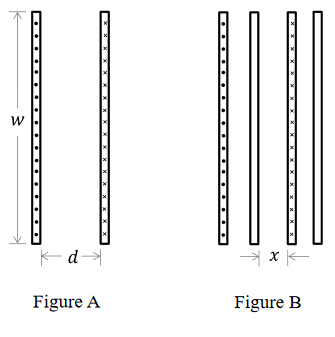
\includegraphics[width=0.5\textwidth]{Sheets.png}
	\end{center}
\end{figure}

(\textit{Source: Speliotopoulos Fall 2014 Final, Problem 6})

\subsection{Transformers: the less-cool kind}

A solenoid of length $l$ and cross-sectional area $A$ is made of $N_p$ turns of a weakly resistive conducting wire.
\begin{itemize}
	\item[(a)] Calculate the self-inductance $L$ of the solenoid.
	\item[(b)] Calculate the energy $U$ stored in this inductor when a current $I$ passes through it.
	\item[(c)] If this solenoid is used as the primary coil of an ideal transformer (as shown), what is the ratio of the currents $I_p$ and $I_s$ passing in the 2 coils?
	\item[(d)] What is the number of turns $N_s$ required on the secondary coil in order to transform 110 V into 15 V? Use $N_p=110$.
\end{itemize}
\begin{figure}[h]
	\begin{center}
		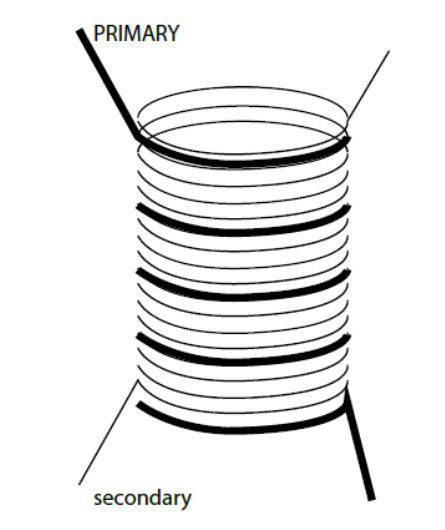
\includegraphics[width=0.3\textwidth]{Transformer.png}
	\end{center}
\end{figure}

(\textit{Source: Bordel Fall 2012 Final, Problem 7})

\end{document}
